% Standalone supplementary information document, built only by `just submit`.
% ISME requires supplementary material as a file separate from the main
% manuscript; this wraps sections/supplementary.tex in its own document so it
% carries a title block, matching line numbering and spacing, and its own
% bibliography. In the default (combined) build this file is unused and
% main.tex inputs sections/supplementary.tex directly.

%!TEX root = ../main.tex

%--------------------------------------------------------%
% DOCUMENT CLASS
%--------------------------------------------------------%

  \documentclass[letterpaper,12pt]{article}

%--------------------------------------------------------%
% TITLE SECTION
%--------------------------------------------------------%

  %Abstract
  \usepackage{abstract}
  \renewcommand{\abstractnamefont}{\normalfont\bfseries}
  \renewcommand{\abstracttextfont}{\normalfont\small\itshape}

  %Title
  \usepackage{titlesec}

  %Authors
  \usepackage{authblk}

  %Date
  \usepackage{datetime2}
  \DTMsetstyle{mdyy} % US date format

%--------------------------------------------------------%
% HEADERS & FOOTERS
%--------------------------------------------------------%

  \pagestyle{plain}

%--------------------------------------------------------%
% MACROS
%--------------------------------------------------------%

  \providecommand{\keywords}[1]{\textbf{\textit{Keywords---}} #1}

%--------------------------------------------------------%
% MATH SUPPORT
%--------------------------------------------------------%

  \usepackage{amssymb}
  \usepackage{amsthm}
  \usepackage{newtxmath}
  \usepackage{mathtools}
  \usepackage{blkarray, bigstrut}

%--------------------------------------------------------%
% FONTS
%--------------------------------------------------------%

  \usepackage{microtype}
  \usepackage{newtxtext}

%--------------------------------------------------------%
% LINES
%--------------------------------------------------------%

  \usepackage{setspace}
  \usepackage{lineno}
  \usepackage[table,x11names]{xcolor}
  \usepackage{enumitem}
  \setlist{nosep}
  \setlist[itemize]{leftmargin=*}

%--------------------------------------------------------%
% MARGINS
%--------------------------------------------------------%

  \usepackage[top=1in, bottom=1in, left=1in, right=1in]{geometry}

%--------------------------------------------------------%
% COMMENTS
%--------------------------------------------------------%

  \usepackage[colorinlistoftodos]{todonotes}
  \usepackage{soul}
  \usepackage{comment}
  \usepackage{xcolor}
  \usepackage{xcolor}
  \usepackage{framed}

  \newif\ifshowalts
  \showaltstrue

  \newenvironment{alttext}[1][]{
    \ifshowalts
      \begin{framed}
      \noindent\textbf{ALT TEXT}\ifx\\#1\\\else\ \textbf{(#1)}\fi\par
      \vspace{0.5ex}
    \else
      \expandafter\comment
    \fi
  }{
    \ifshowalts
      \end{framed}
    \else
      \endcomment
    \fi
  }
  \newcommand{\altsentence}[2]{%
  \ifshowalts
    \begin{alttext}[#1]
    #2
    \end{alttext}
  \fi}

%--------------------------------------------------------%
% ACRONYMS
%--------------------------------------------------------%

  \usepackage[nohyperlinks,nolist]{acronym}

%--------------------------------------------------------%
% GRAPHICS
%--------------------------------------------------------%

  \usepackage{graphicx}
  \usepackage{caption}
  \usepackage{subcaption}
  \graphicspath{{figures/}}
  \usepackage{float}
  \usepackage{printlen}
  \usepackage[section]{placeins}

%--------------------------------------------------------%
% TABLES
%--------------------------------------------------------%

  \usepackage{longtable}
  \newcommand{\sym}[1]{\rlap{#1}}
  \usepackage{tabularx}
  \newcolumntype{L}[1]{>{\raggedright\arraybackslash}p{#1}}
  \newcolumntype{C}[1]{>{\centering\arraybackslash}p{#1}}
  \newcolumntype{R}[1]{>{\raggedleft\arraybackslash}p{#1}}
  \usepackage{makecell}
  \usepackage{relsize}
  \usepackage{multirow}
  \usepackage{pdflscape}

%--------------------------------------------------------%
% REFERENCES (load hyperref last!)
%--------------------------------------------------------%

  \usepackage{csquotes}
  \usepackage[
    style=nature,
    doi=true,
    url=false,
    backend=biber,
    sorting=none,
    maxbibnames=3,
    minbibnames=3,
  ]{biblatex}
  \DeclareFieldFormat{doi}{\url{https://doi.org/#1}}
  \bibliography{references.bib}
  % xr-hyper must precede hyperref; resolves \ref across main.tex <-> supplement.tex
  \usepackage{xr-hyper}
  \usepackage{hyperref}
  % let long URLs wrap at slashes, hyphens and dots instead of running into the margin
  \def\UrlBreaks{\do\/\do-\do.}


% Resolves \ref to main-text figures and tables from build/main.aux. This needs
% main.tex compiled first, which `just submit` handles. Do NOT compile this file
% on Overleaf: only the main document is built there, so build/main.aux will not
% exist and every main-text reference will render as ??.
\externaldocument{build/main}

\begin{document}

\thispagestyle{empty}

\begin{center}
  {\huge Supplementary Information}\\[0.8cm]
  {\large Data coherence over data volume drives generalisable genome-based
  prediction of microbial carbon utilisation}\\[0.8cm]
  Dileep Kishore, Priya Ranjan, Christopher Neely, Mikaela Cashman,
  William Riehl, Marcin P. Joachimiak, Janaka N. Edirisinghe,
  Jos\'{e} P. Faria, Myra B. Cohen, Zahmeeth Sakkaff, Pamela Weisenhorn,
  Dale A. Pelletier, Mitchel J. Doktycz, Robert W. Cottingham,
  Christopher S. Henry, Adam P. Arkin, Paramvir S. Dehal\\[0.5cm]
  Corresponding author: Paramvir S. Dehal (psdehal@lbl.gov)
\end{center}

\vspace{1cm}

\linenumbers
\setlength\linenumbersep{15pt}
\renewcommand\linenumberfont{\normalfont\footnotesize\sffamily\color{gray}}
\modulolinenumbers[1]

\doublespacing

%!TEX root = ../main.tex

\section*{Supplementary Material}

  \renewcommand{\thefigure}{S\arabic{figure}}
  \setcounter{figure}{0}

  \renewcommand{\thetable}{S\arabic{table}}
  \setcounter{table}{0}

% ============================================================
%   SUPPLEMENTARY TEXT
% ============================================================

\subsection*{Supplementary Text S1: Dataset Descriptions}

We harmonised four experimental carbon source utilisation datasets spanning phylogenetically and ecologically diverse bacteria; analyses used the 15 phenotypes shared across all four datasets (Table~\ref{tab:dataset_overview}).
ATLeaf~\cite{Schafer2023-nk} tested \textit{Arabidopsis thaliana} leaf-surface isolates on minimal agar medium.
Biolog~\cite{BiologDatasetCitation} was compiled from multiple published studies; growth calls derive predominantly from Biolog Phenotype MicroArray colourimetric tetrazolium assays in 96-well plates, with a subset from other published growth-assay formats, and per-strain sources are given in the deposited metadata~\cite{ZenodoDeposit}.
Marine~\cite{Gralka2023-ft} assessed heterotrophic marine bacteria.
Populus~\cite{PopulusDatasetCitation} is a Biolog carbon-source assay of ORNL Plant-Microbe Interfaces isolates from the \textit{Populus deltoides} rhizosphere and endosphere, recording optical density in MOPS minimal medium.
Because of its small sample size and narrow phylogenetic breadth, Populus was excluded from selected feature-stability comparisons.

Generic carbon-source names such as ``glucose'' or ``serine'' do not specify stereochemistry, and the four datasets did not always assay the same isomer under the same name, so each phenotype was bound to one explicit source substrate, retaining the physiologically utilised isomer where a dataset assayed more than one.
Identities were verified against Table~S1 of Sch\"afer et al.~\cite{Schafer2023-nk} for ATLeaf, Supplementary Table~2 of Gralka et al.~\cite{Gralka2023-ft} for Marine, and the Biolog PM1 and PM2A plate maps for the Biolog and Populus assays. \texttt{substrate\_identity\_common15.csv} in the Zenodo deposit~\cite{ZenodoDeposit} records the resulting bindings, with a companion table covering all 240 carbon sources.
Two cases warrant comment.
The Marine \emph{alanine} well contained DL-alanine whereas the other three datasets assayed L-alanine; a racemate well scores positive if either enantiomer is utilised, so the Marine column is a union trait rather than a different trait.
For \emph{glucose}, the Populus alpha-D-glucose well was retained over the L-glucose well, which these taxa do not catabolise; the anomeric distinction is immaterial in solution because the free sugar interconverts by mutarotation, whereas for methyl glucosides and galactosides the locked acetal makes the two anomers separate traits taken up by different systems.

\subsection*{Supplementary Text S2: Genome Quality Assessment}

Genome quality was assessed with CheckM2 v1.1.0~\cite{Chklovski2023CheckM2} and recorded as a covariate rather than applied as an exclusion criterion, so that performance reflects the assemblies a user would realistically supply.
Of the 755 modelled strains with a CheckM2 record, 689 met the MIMAG high-quality thresholds (completeness $\geq$90\%, contamination $\leq$5\%) and 732 met the medium-quality thresholds (completeness $\geq$50\%, contamination $\leq$10\%).
Repeating the CatBoost KOFAM analysis for all 15 shared phenotypes with training, validation, and test sets each restricted to a quality tier left balanced accuracy essentially unchanged.
Relative to the unfiltered data, the high-quality tier shifted it by a median of $+0.004$ under random splits (75 phenotype-fold pairs, Wilcoxon $p = 0.03$) and $+0.015$ under cross-dataset splits (58 pairs, $p = 0.003$), and the medium-quality tier by $-0.000$ ($p = 0.72$) and $+0.005$ ($p = 0.05$).
These shifts are more than an order of magnitude smaller than the gap between random and cross-dataset splits, so genome quality filtering does not alter any conclusion reported here.

As an independent secondary audit, we measured pangenome completeness as the fraction of species-specific core genes detected by MMseqs2~\cite{Steinegger2017MMseqs2} at 90\% identity, 80\% coverage, and E-value $10^{-3}$.
353 of the 394 assessed genomes with both a species assignment and a core-gene set (89.6\%) exceeded 90\% completeness (Figure~\ref{fig:pangenome_completeness}).

\subsection*{Supplementary Text S3: Model Selection and Evaluation Details}

\paragraph*{GapMind pathway annotation.}
Carbon-utilisation pathway completeness was computed with GapMind~\cite{Price2022GapMindCarbon,Price2020GapMind} from the PaperBLAST suite (\url{https://github.com/morgannprice/PaperBLAST}, commit 1033662, accessed May 2025).
For each pathway step, candidate genes were found by USEARCH v11.0.667~\cite{Edgar2010} against curated reference databases (minimum 30\% identity) and by HMMer v3.3.1 profile search~\cite{Eddy2011}.
Reverse searches validated candidates, and required-step matches, alternative routes, and isofunctional enzymes determined the 0--2 pathway-completeness scores and the Methods thresholds.

\paragraph*{Model family and hyperparameters.}
We compared gradient-boosted trees, regularised-linear and projection methods, Random Forest, and a phylogeny-aware model across 15 phenotypes and four evaluation regimes.
88\% of phenotype--regime cells tied within 0.05 balanced accuracy, with boosted trees strongest and Random Forest the only consistent under-performer (Table~\ref{tab:best_models_counts}).
This comparison used one protocol without early stopping, so its absolute values differ by $\sim$0.02 BA from the early-stopping CatBoost results.
CatBoost was retained at 1000 iterations, learning rate 0.03, depth 4, L2 regularisation 15, 10\% random feature subsampling, Bayesian bootstrap, and logloss early stopping with patience 50, because further phenotype-specific tuning did not improve accuracy.
The minority-class filter (Methods) was computed on the test subset plotted in each analysis and applied identically to both series in every machine-learning-versus-GapMind comparison (\texttt{scripts/minority\_filter.py}).

\paragraph*{Replicate genomes and random-holdout overlap.}
Among the 755 KOFAM feature profiles entering at least one shared-phenotype split, 17 formed eight exact-duplicate groups, each confined to a single source dataset, so leave-one-dataset-out evaluation contained no exact-vector train--test overlap.
Across random-holdout splits, approximately 1.4\% of test predictions had an identical same-label vector in the training pool and approximately 9\% a nearest training vector at Jaccard $\geq 0.98$ (\texttt{scripts/leakage\_check\_feature\_dup.py}).
Because both pre-processing filters are label-free, applying them across the full dataset rather than per split cannot leak labels, although the retained feature set reflects the pooled feature distribution; classifiers were still fitted on training samples only.

\subsection*{Supplementary Text S4: Histidine Feature Comparison}

Table~\ref{tab:feature_comparison} gives the histidine worked example under full-data and concordant training.
Stable features ranked among the top 10 by mean absolute SHAP value in at least 70\% of 20 runs, with cluster labels denoting SHAP-supervised redundancy groups (Methods).
Under full-data training, core histidine enzymes other than K01712 appeared among dataset-specific stable features but not in the aggregated dataset.
Under concordant training, the cluster containing K01468 (imidazolonepropionase), K01712 (urocanate hydratase), and K05836 (histidine-utilisation repressor) was recovered across datasets, the shared-cluster count rose from 4 to 8, the held-out-alone count fell from 6 to 3, and pathway concentration on map00340 rose from 17\% to 33\%.


The example shared feature column of Table~\ref{tab:main_feature_comparison} shows a shared KO where the two models select the same feature outright, and otherwise a representative KO from each shared redundancy cluster; at most two are listed, so the column is illustrative rather than exhaustive, and it is empty only where no cluster is shared.
Features are ranked by the number of held-out comparisons in which they recur, and those whose redundancy cluster touches the row's KEGG map are listed first; off-pathway transporters or regulators appear only where no shared cluster touches the map (for Glycerol, the glpF facilitator and the glpR repressor; for Arginine, off-pathway choline/betaine and sarcosine-oxidase clusters).
The displayed features do not enter the (\% in pathway) statistic, which scores canonical pathway-map residency across all shared clusters rather than the one or two shown.

% ============================================================
%   FIGURES
% ============================================================

\begin{figure}[h]
\centering
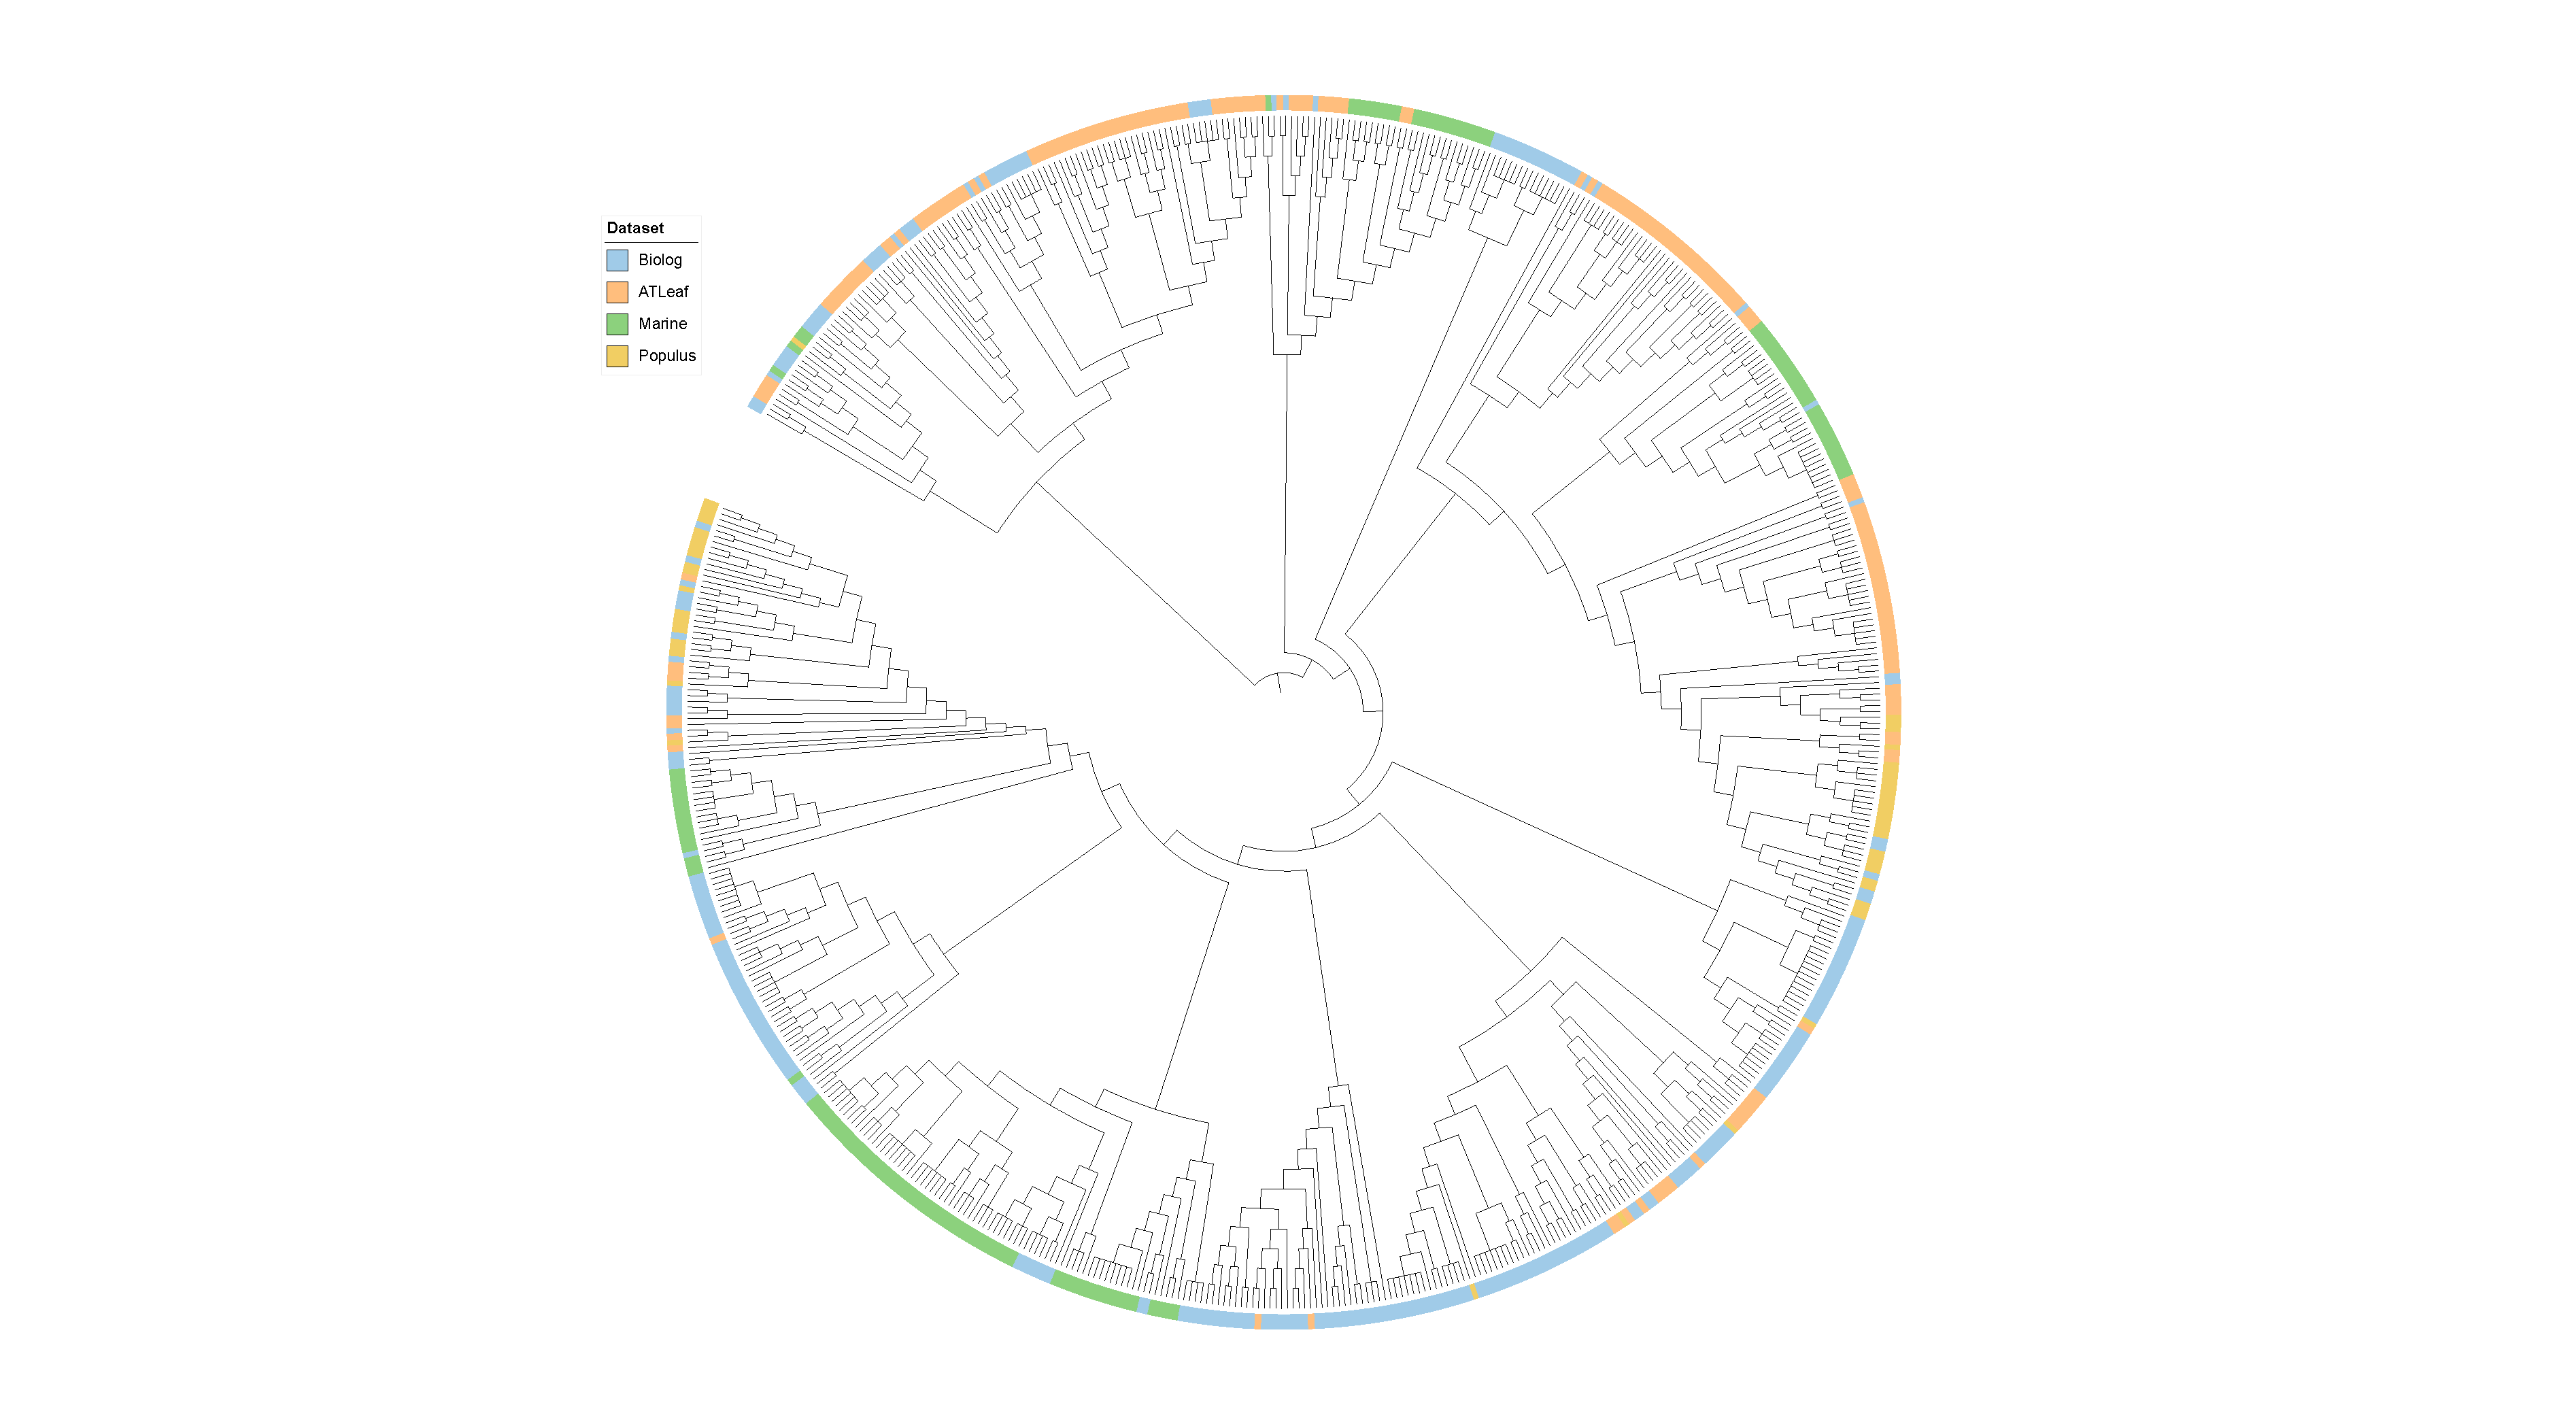
\includegraphics[width=\textwidth]{figure_s1.pdf}
\caption{\textbf{The four datasets span overlapping but unevenly sampled regions of the bacterial tree.}
Of the 819 input strain records, 629 GTDB-placed tips were retained in the pruned Genome Taxonomy Database reference tree~\cite{Parks2018GTDB}, with distances calculated using ETE 3~\cite{HuertaCepas2016ETE3}.
The tree is drawn as a cladogram, so branch lengths are not to scale; phylogenetic distances are reported in Figure~\ref{fig:phylogenetic_distance_splits}.
The inner ring denotes dataset membership and the outer bar the GTDB order, coloured by GTDB class; orders with at least eight tips are labelled with their tip count, and tip labels are omitted for legibility.}
\label{fig:phylogenetic_distribution}
\end{figure}

\begin{figure}[h]
\centering
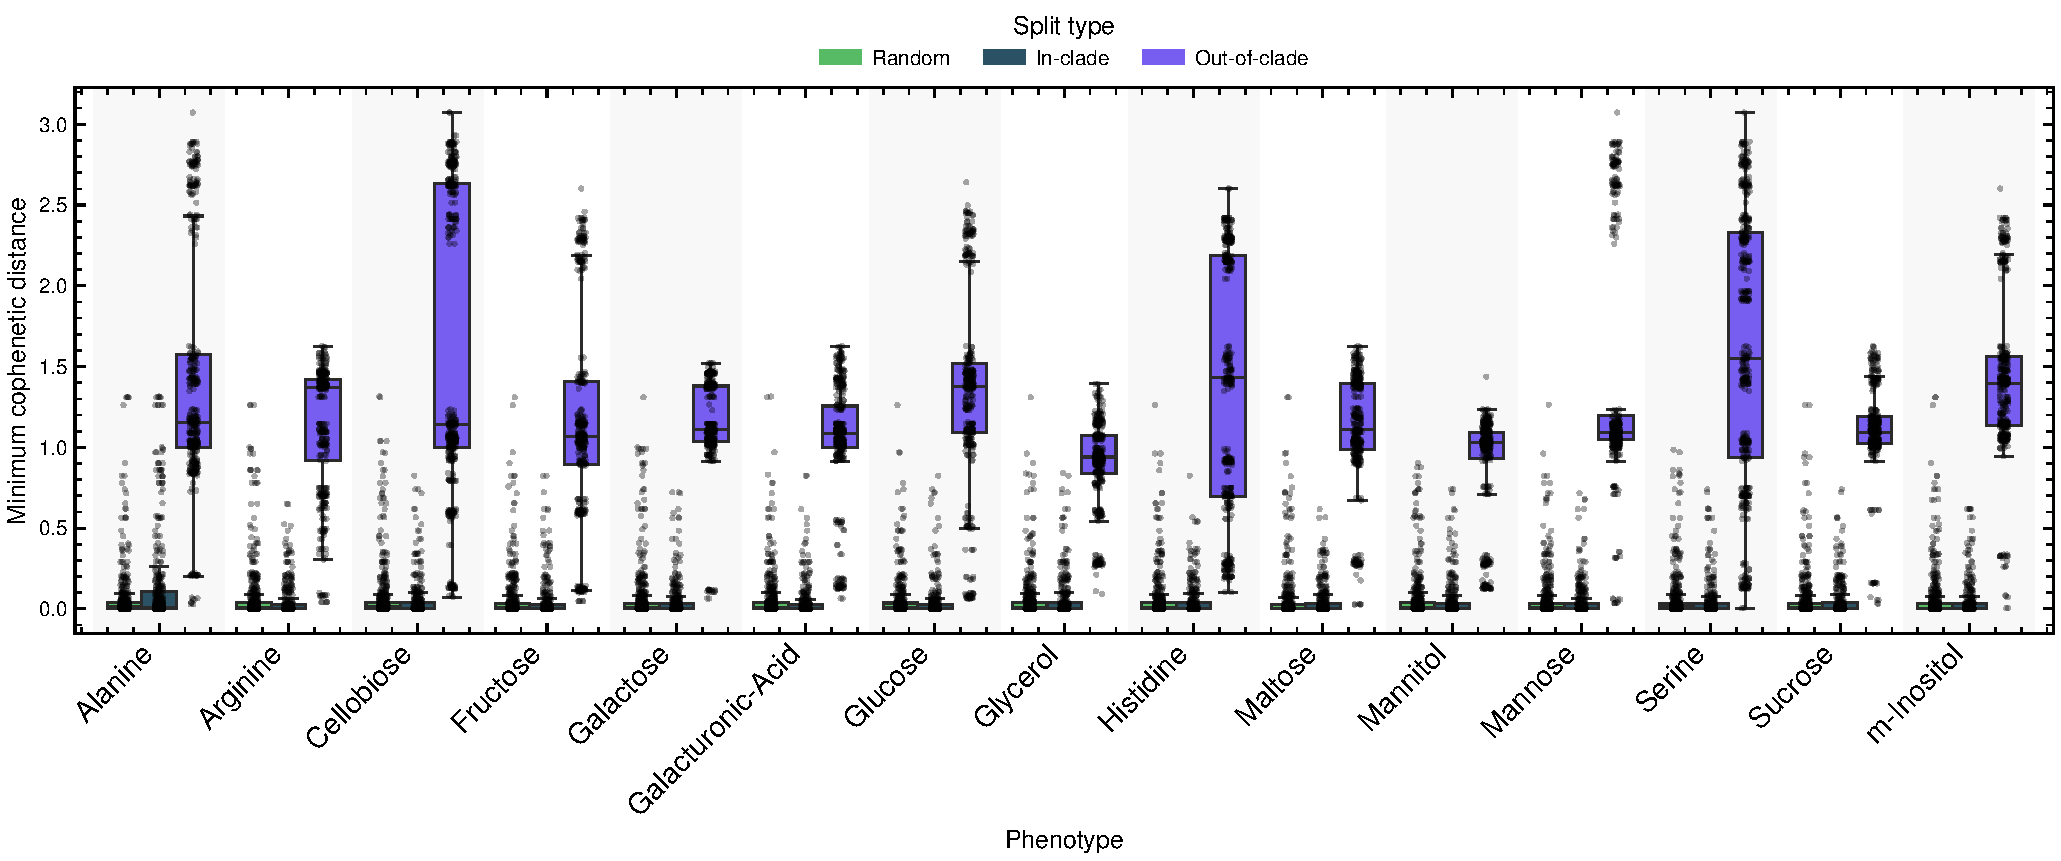
\includegraphics[width=\textwidth]{figure_s2.pdf}
\caption{\textbf{Only out-of-clade splits place test genomes far from their training set.}
Minimum cophenetic distance from each held-out test genome to its training set under random-holdout, in-clade, and out-of-clade splits, pooled across five splits per phenotype for the 15 shared phenotypes.
Boxes are coloured by split type (random, green; in-clade, dark teal; out-of-clade, purple), show the median and interquartile range, points are individual test genomes (random $n=8{,}289$; in-clade $n=5{,}595$; out-of-clade $n=6{,}212$).
Random-holdout and in-clade test genomes lie close to the training set (medians 0.009 and 0.000), whereas out-of-clade splits produce much larger distances (median 1.109), validating the intended separation of the evaluation regimes in Figure~\ref{fig:ml_performance}.}
\label{fig:phylogenetic_distance_splits}
\end{figure}

\begin{figure}[h]
\centering
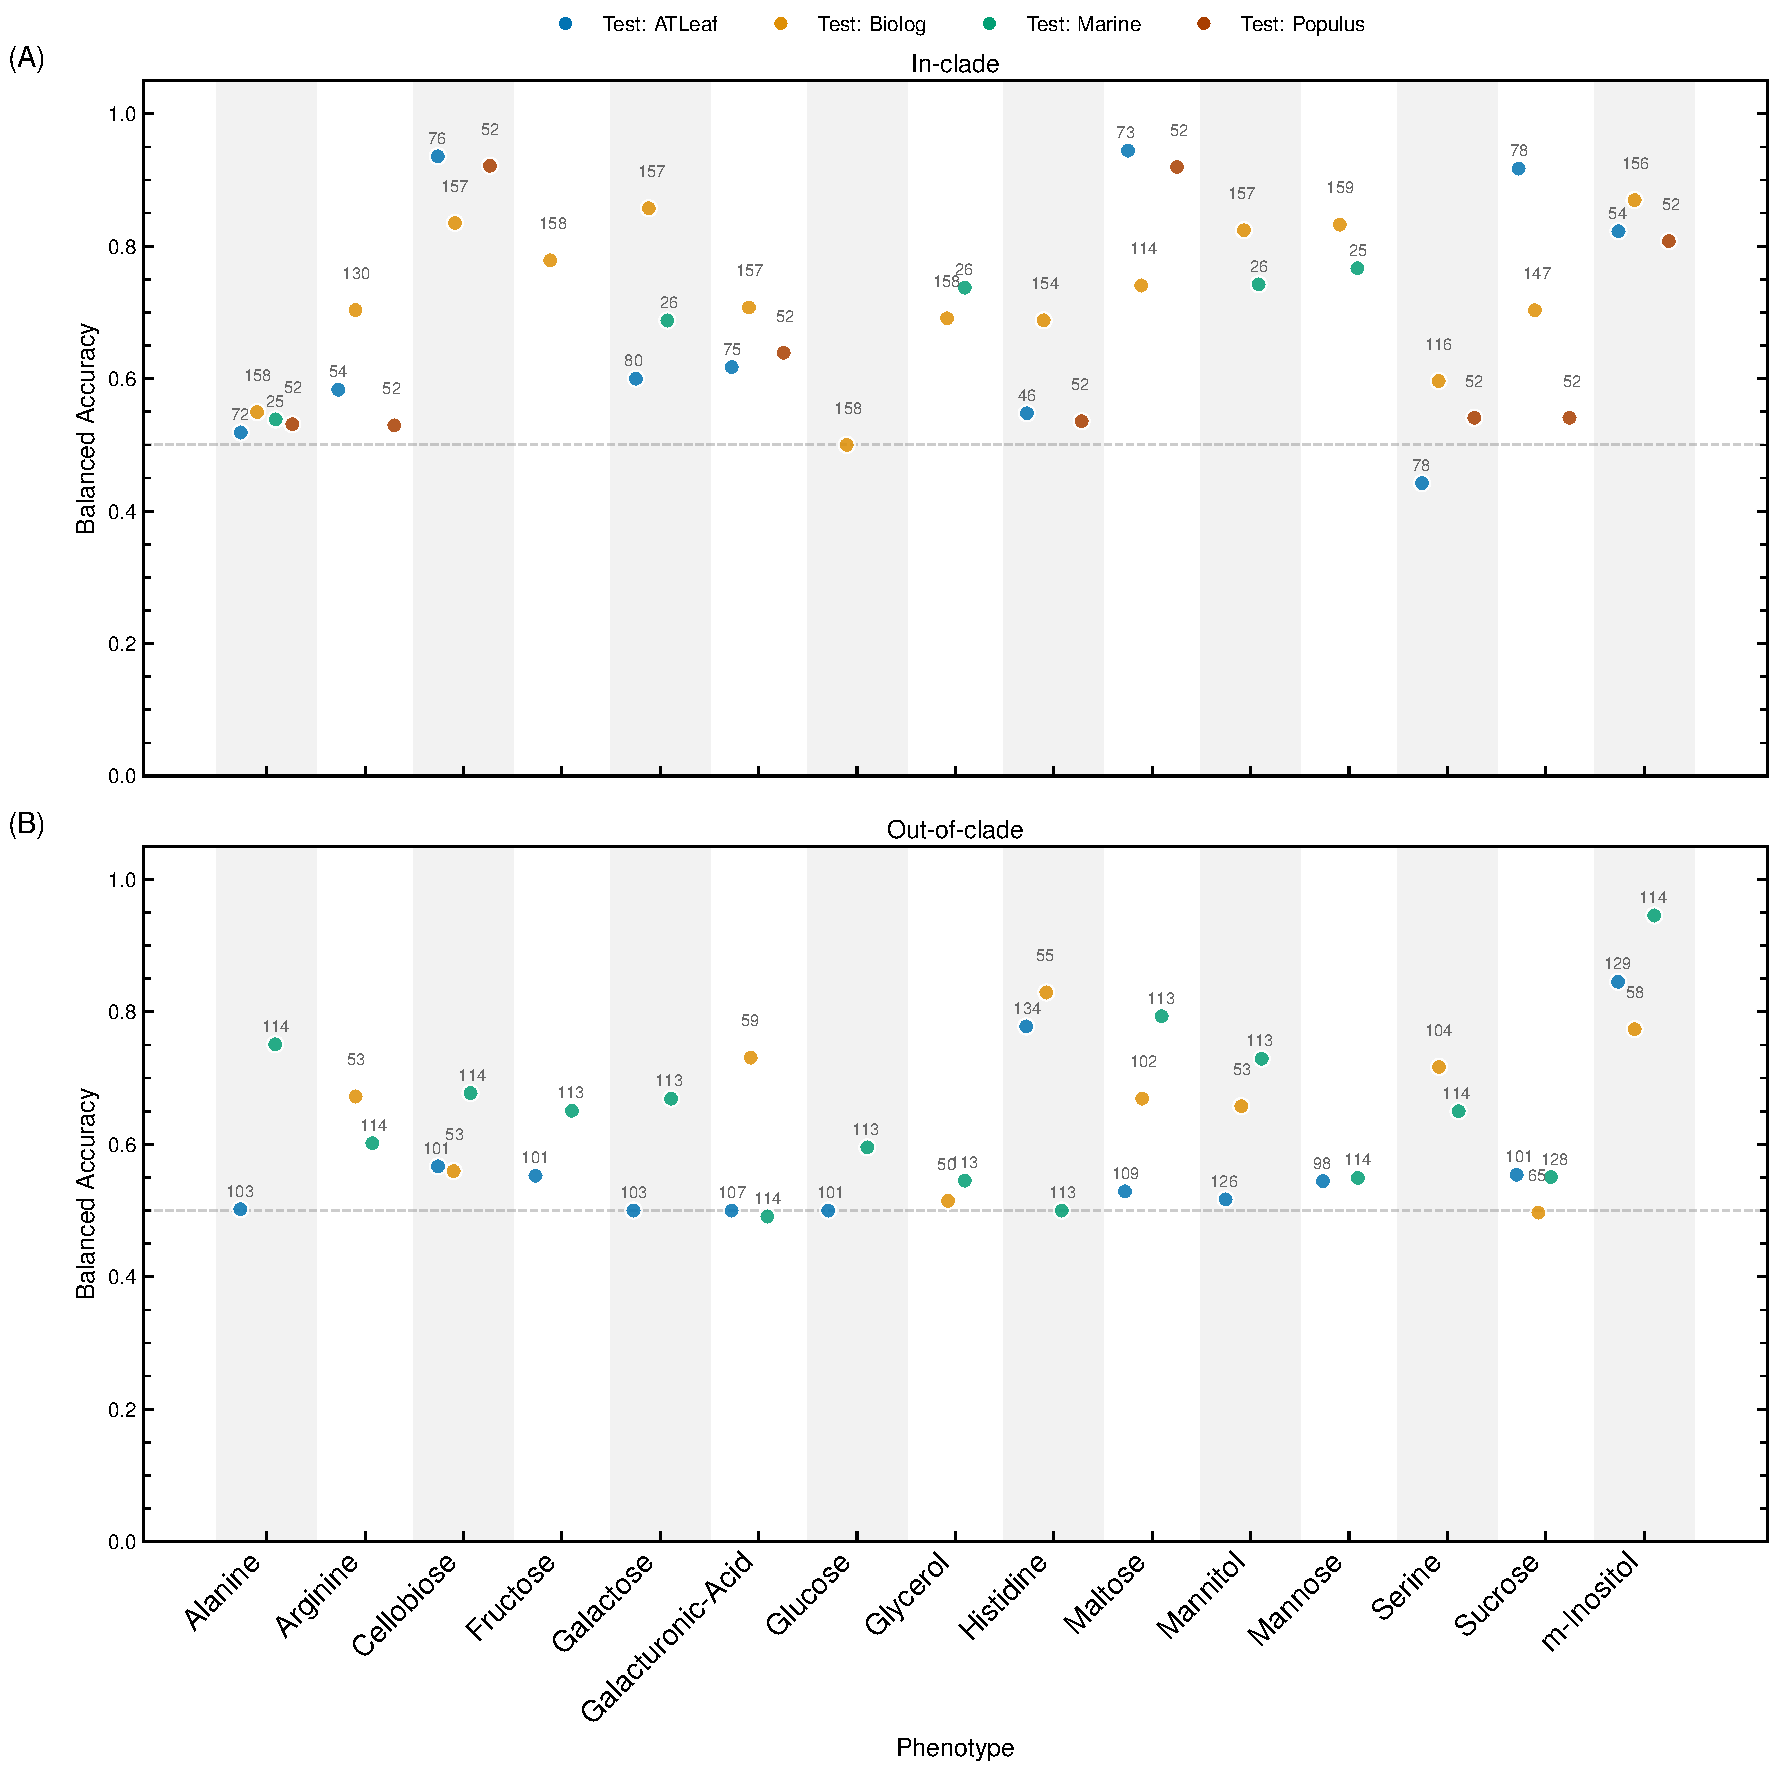
\includegraphics[width=\textwidth]{figure_s3.pdf}
\caption{\textbf{Cross-dataset accuracy is lower for genomes without close training relatives.}
CatBoost balanced accuracy using KOFAM features across four leave-one-dataset-out combinations.
(\textbf{A}) In-clade, test samples sharing a cluster with at least two training samples; (\textbf{B}) out-of-clade, test samples sharing a cluster with fewer than two, using the Figure~\ref{fig:ml_performance}C clustering procedure.
Points are coloured by held-out test dataset.
Cells with fewer than 10 test or minority-class samples were excluded (44 of 120, including all Populus-held-out out-of-clade cells).
Mean out-of-clade balanced accuracy was lower than in-clade accuracy (0.621 versus 0.701).
Numerals give test-subset sizes.}
\label{fig:in_clade_out_clade_performance}
\end{figure}

\begin{figure}[h]
\centering
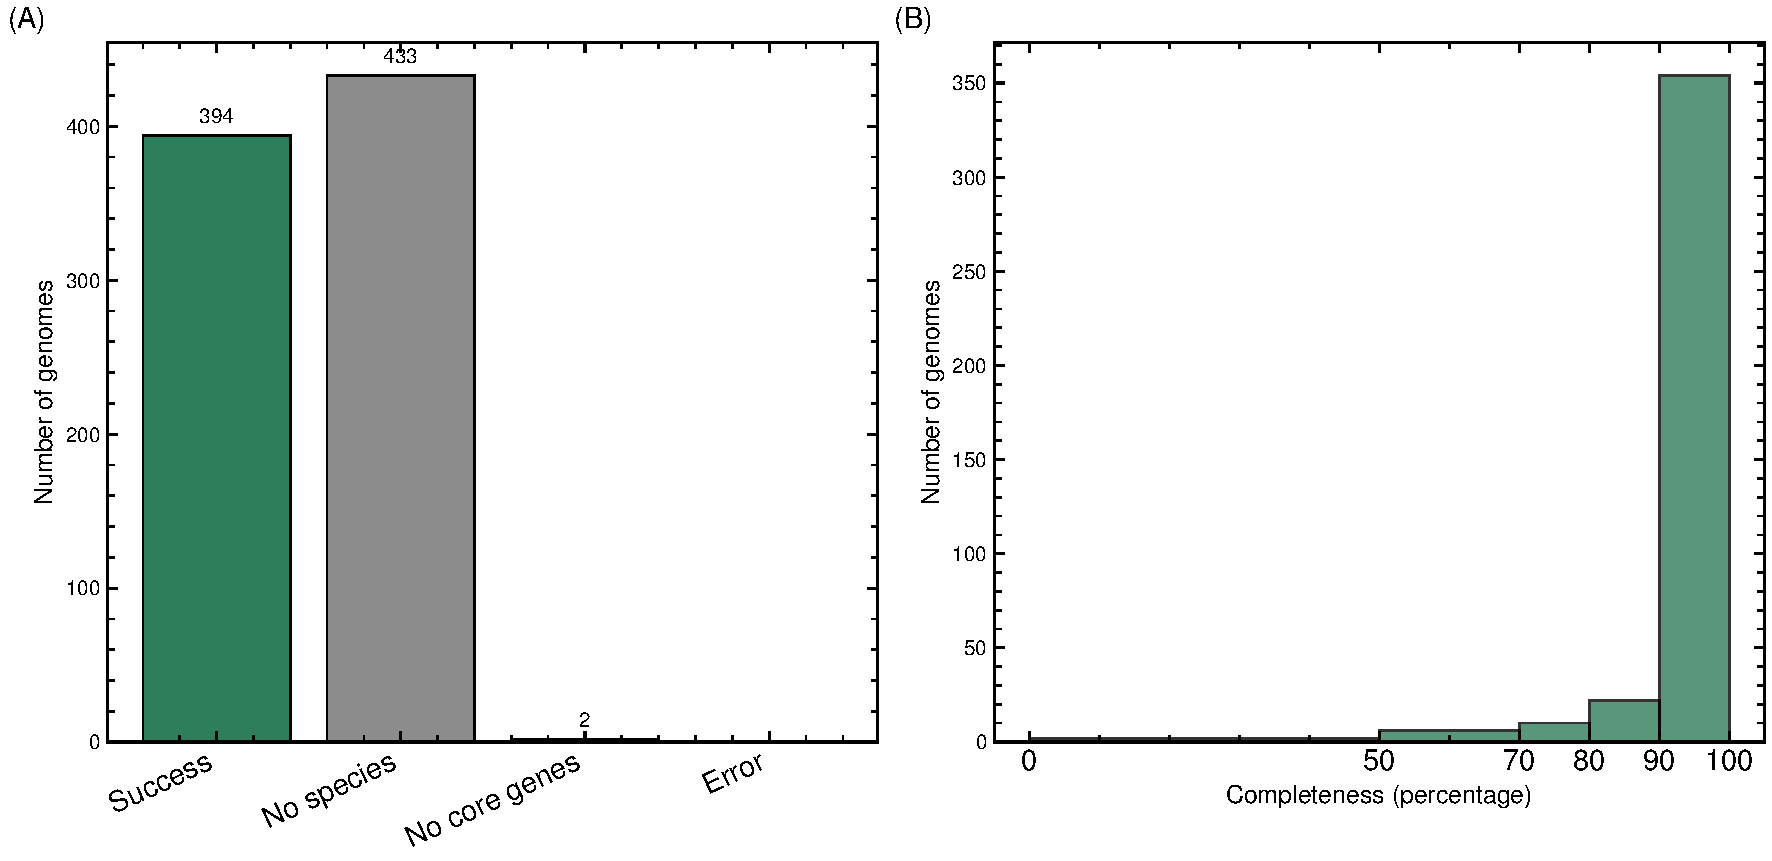
\includegraphics[width=\textwidth]{figure_s4.pdf}
\caption{\textbf{Pangenome completeness could be assessed for a subset of genomes, nearly all of which were near-complete.}
Completeness was the fraction of species core genes detected by MMseqs2 at 90\% identity, 80\% coverage, and E-value $10^{-3}$.
(\textbf{A}) Assessment status.
(\textbf{B}) Completeness among successfully assessed genomes, most of which exceeded 90\%.}
\label{fig:pangenome_completeness}
\end{figure}

\subsection*{Supplementary Text S5: Concordant Training Under the KOFAM Feature Space}

GapMind concordance selected training samples, whereas KOFAM annotations supplied model features, decoupling the selection rule from the feature space.
Under the same KOFAM feature space, concordant training improved cross-dataset balanced accuracy on concordant test samples for most phenotype--split combinations (Figure~\ref{fig:kofam_concordant}).
The feature-recovery analysis nevertheless remains biologically related to the selection rule, since GapMind and KOFAM annotate the same genomes.
However, GapMind scores curated reference proteins rather than KEGG modules, SHAP stability across datasets is not entailed by the selection rule, and several phenotypes recovered predominantly off-map features.
A size and class-matched random-subset control recovered $0.38 \pm 0.03$ shared clusters (mean $\pm$ SD across ten draws), similar to full-data training (0.5) and below concordant training (1.3), indicating that the stability gain was specific to concordance rather than sample count (\texttt{scripts/figure5/figure5b\_random\_control.py}).

Raw, uncorrelated GapMind features were used for the rule-reconstruction reference (Figure~\ref{fig:concordant_analysis}A) and the phenotype-filtered comparison (Figure~\ref{fig:improvement_strategies}D) because the standard 0.95 correlation filter collapses repeated phenotype-prefixed representations of the same gene and can deplete individual pathway feature sets.
Because these features are the evidence the concordance rule itself is computed from, this reference bounds how far that rule can be reconstructed by the ML model from its own inputs, and is not an estimate of annotation quality.

Feature selection within the combined matrix indicates why concatenating annotation types did not improve transfer (Figure~\ref{fig:dataset_characteristics}C).
RAST subsystem terms contribute 62.6\% of its 17,152 correlation-filtered features, KOFAM 31.8\%, and GapMind only 5.7\%; yet among the top ten features by mean absolute SHAP value across the cross-dataset splits, GapMind terms account for 43.0\% of selections, a 7.6-fold enrichment, RAST terms for 26.8\%, a 0.4-fold depletion, and KOFAM terms in proportion to their share.
The comprehensive set therefore inherits the same dependence on curation as the phenotype-filtered set without its accuracy: the roughly 34 curated features of a single phenotype outperformed all 17,152 combined features under cross-dataset evaluation (Figure~\ref{fig:improvement_strategies}D).

\begin{figure}[ht]
\centering
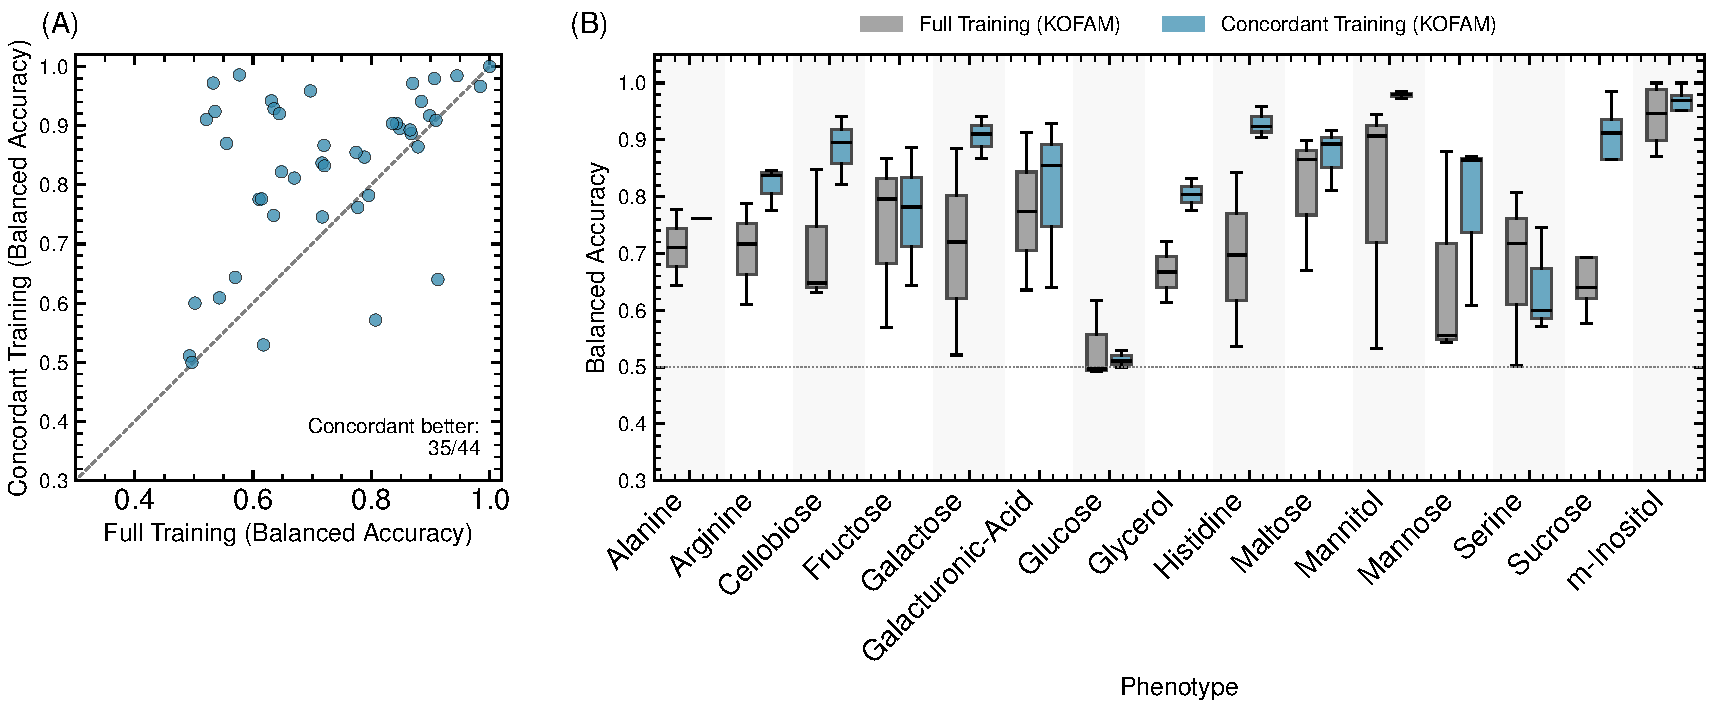
\includegraphics[width=0.90\textwidth]{figure_s5.pdf}
\caption{
\textbf{Concordant training improves cross-dataset generalisation under KOFAM features.}
(\textbf{A}) Cross-dataset balanced accuracy of concordance-trained versus full-data KOFAM models on concordant test samples; each point is one phenotype--split combination ($n = 44$), and the annotation gives the number of combinations on which concordant training was better.
(\textbf{B}) Per-phenotype distributions for full-data (grey) and concordant (purple) training; boxes show the median and interquartile range, and the dotted line marks the 0.5 chance level.
Each box summarises the one to four cross-dataset splits available for that phenotype, so boxes for phenotypes with a single split appear as a line.
}
\label{fig:kofam_concordant}
\end{figure}

\subsection*{Supplementary Text S6: Learning Curves for the Shared Phenotypes}

Across the 15 shared phenotypes, concordance-trained KOFAM performance approached its all-available-sample value within 50 to 100 training samples (Figure~\ref{fig:sample_size_phenotypes}).
Under cross-dataset evaluation, 11 of 15 phenotypes reached 90\% of their all-sample balanced accuracy with 50 samples and 14 of 15 with 100, fructose alone requiring 200.
Median performance at 50 samples was 93.6\% of the all-sample value for concordant training and 91.0\% for full-data training.
Early saturation does not by itself indicate a well-predicted phenotype.
The five phenotypes saturating with 25 cross-dataset samples had a median all-sample balanced accuracy of 0.63, against 0.73 for the remainder, and cross-dataset gains between 25 samples and the full set were larger for phenotypes that ultimately performed better (Spearman $\rho = 0.78$, $p = 0.0007$).
Glucose, for example, saturated immediately at a balanced accuracy of 0.51.
Additional samples therefore helped most where transfer was already succeeding, consistent with a representational rather than a statistical limit on the phenotypes that failed to transfer.

\begin{figure}[ht]
\centering
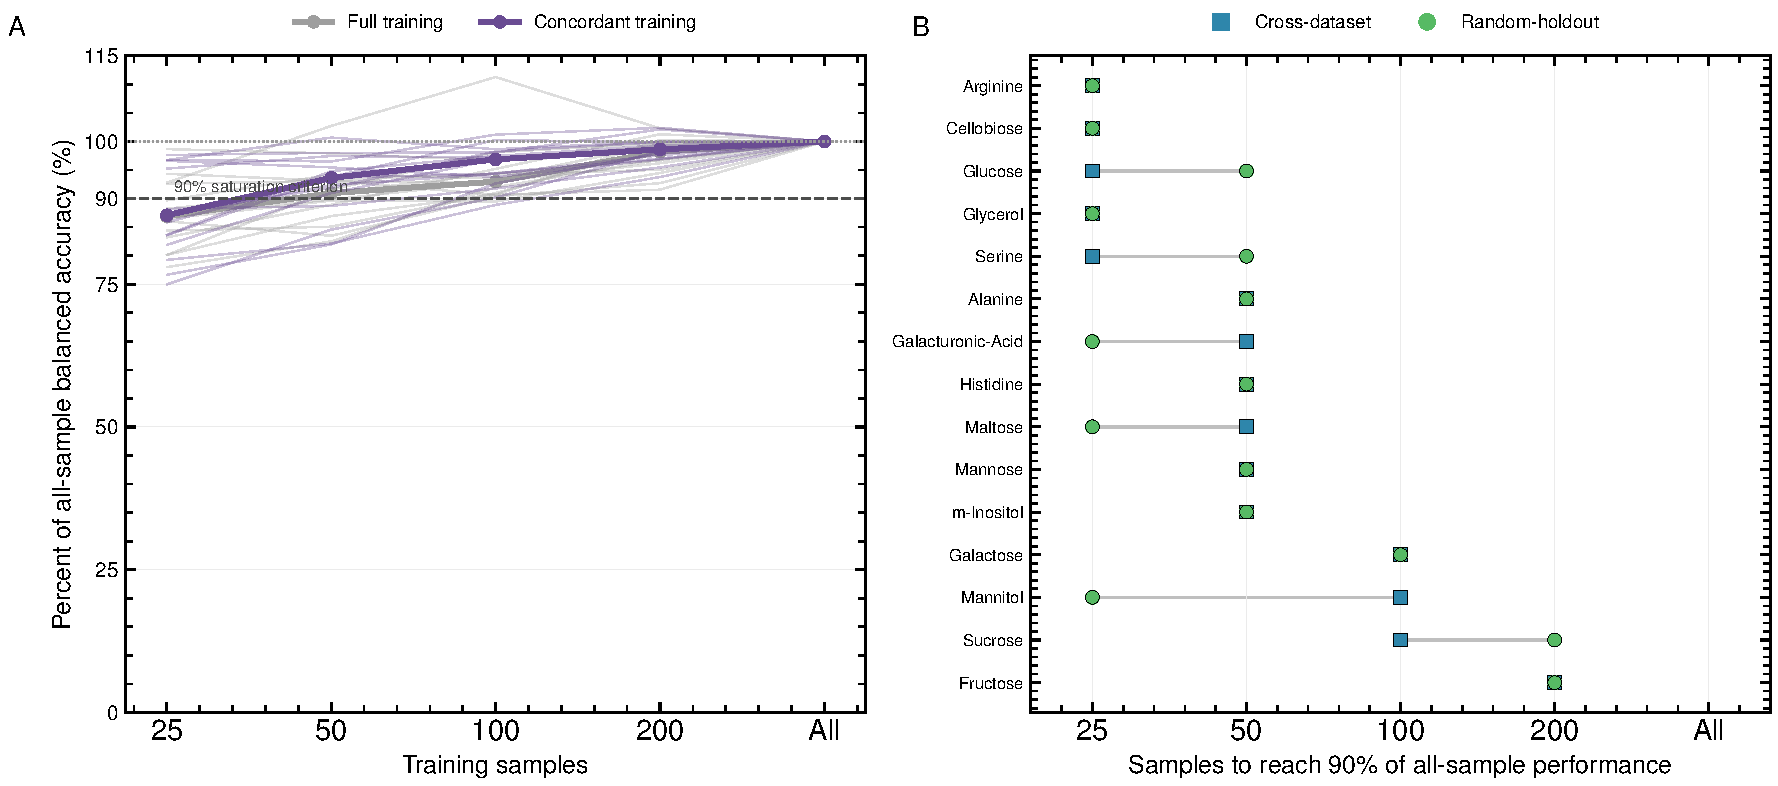
\includegraphics[width=\textwidth]{figure_s6.pdf}
\caption{
\textbf{Cross-dataset performance saturates at 50--100 training samples for most phenotypes.}
(\textbf{A}) Cross-dataset balanced accuracy at each training-set size, expressed as a percentage of the same phenotype's all-sample value, for full-data (grey) and concordant (purple) training.
Thin lines are individual phenotypes and bold lines their medians; the dashed line marks the 90\% saturation criterion and the dotted line the all-sample value.
Values above 100\% arise where an intermediate training-set size outperformed the full set.
(\textbf{B}) Smallest training-set size at which each phenotype reached 90\% of its all-sample performance under cross-dataset (blue squares) and random-holdout (green circles) evaluation, ordered by the cross-dataset value.
Points are means across repeats and across the splits available for each phenotype, at requested sizes of 25, 50, 100, 200, and all available samples.
}
\label{fig:sample_size_phenotypes}
\end{figure}

\subsection*{Supplementary Text S7: SHAP-Supervised Redundancy Clustering Procedure}

Stable features were identified with a fixed 500-iteration CatBoost model trained without early stopping, using 20 random seeds per phenotype--dataset configuration.
A feature was designated stable when it ranked among the top ten by mean absolute SHAP value in at least 70\% of those runs.

Because correlated KOs can represent the same predictive signal, the stable-feature comparisons in Figures~\ref{fig:misclassification_diagnosis}C and~\ref{fig:concordant_analysis}B intersect clusters rather than raw KOs.
For each phenotype, the union of stable KOs was clustered on the pooled concordant feature matrix across all four datasets with \texttt{shap.utils.hclust} in SHAP v0.50.0~\cite{Lundberg2017SHAP,Lundberg2020TreeSHAP,SHAPhclustDocs}.
Supplied with the phenotype labels, the routine fitted a univariate XGBoost model of the phenotype from each KO, then a second model predicting that first-stage output from every other KO; each directional distance was $1-R^2$.
The smaller directional distance for each KO pair formed a single-linkage matrix, which was cut at a distance threshold of 0.5.

For alanine, mannose, and serine, stable features from different concordance-trained models did not enter the same cluster but remained correlated within some held-out datasets (for mannose, transporters K10441 and K10545 at $|r|=0.67$ in concordant ATLeaf samples).
These features were heterogeneous carbohydrate-utilisation and accessory genes rather than one shared pathway, indicating a broader, less substrate-specific mode of transfer; for alanine, GapMind's pathway definition encodes only transport, so concordance reflects uptake rather than catabolic coverage.

\subsection*{Supplementary Text S8: Reliability and Experiment-Prioritisation Details}

CatBoost probabilities were not post hoc calibrated, so confidence ranked predictions only.
Expected calibration error used ten equal-width bins, pooled across phenotypes for each model.
Neither mean confidence nor the fraction of predictions (with confidence of at least 0.8) predicted per-phenotype cross-dataset balanced accuracy across the 15 phenotypes (Spearman $\rho$ between $-0.18$ and $-0.05$, both $p > 0.5$).

Feature-space novelty was the mean Jaccard distance from a held-out genome to its five nearest training genomes in KOFAM space.
The high-novelty strategy took the candidates ranked highest on this measure; the diversity strategy took candidates evenly spaced along the same ranking.
Each eligible held-out dataset was split approximately 50:50 into candidate and evaluation pools, stratified where possible, and 25 candidate labels were added to the concordant training set.
Models used 120 CatBoost iterations, depth 4, and learning rate 0.05 without evaluation-set early stopping, across three seeds and four held-out datasets.
Because the random baseline also adds labels from the held-out dataset, it carries the benefit of initial exposure, and the other strategies are credited only with improvement beyond it.
After averaging seeds within 23 phenotype--held-out-dataset cells, low-confidence selection exceeded random selection ($p=0.024$, BH-adjusted $q=0.052$); across the six phenotype means, four favoured low-confidence selection and the paired test was not significant ($p=0.156$).

\subsection*{Supplementary Text S9: Composite Confidence Weighting}

The composite score used to weight training and validation samples (Figure~\ref{fig:improvement_strategies}B) was calculated as follows:
\begin{equation*}
    y_{\mathrm{soft}} = w_{\mathrm{phylo}} \cdot \mathrm{phylo} + w_{\mathrm{gap}} \cdot \mathrm{GapMind} + w_{\mathrm{exp}} \cdot \mathrm{exp},
\end{equation*}
Within each split, the phylogenetic component was the mean experimental label among the $k=3$ nearest training genomes and therefore took values 0, $1/3$, $2/3$, or 1.
The training genome was excluded from its own neighbours.
The experimental component was the binary phenotype label used only for training and validation-set quality assessment.
GapMind categories mapped to six numeric levels: complete, 1.0; likely complete, 0.9; steps missing medium, 0.6; steps missing low, 0.3; not present, 0.1; and no evidence or uncategorized, 0.0.
After clipping $y_{\mathrm{soft}}$ to $[0.01,0.99]$, every scored sample was retained and assigned the recall-prioritised weight
\begin{equation*}
    s_i =
    \begin{cases}
        y_{\mathrm{soft},i}, & \mathrm{exp}_i = 1,\\
        \max\left(0.01, 2\left|y_{\mathrm{soft},i}-0.5\right|\right), & \mathrm{exp}_i = 0.
    \end{cases}
\end{equation*}
The asymmetric weighting prioritised recall while ensuring that every phylogenetic conflict reduced confidence.
In the mechanism-free setting, complete phylogenetic conflicts remained in training with weights 0.60 for positive labels and 0.20 for negative labels, while complete agreements received 0.99 and 0.98, respectively.
Four weight configurations $(w_{\mathrm{phylo}}, w_{\mathrm{gap}}, w_{\mathrm{exp}})$ were evaluated: the mechanism-free $(0.40, 0.00, 0.60)$ and three GapMind-weighted settings $(0.20, 0.30, 0.50)$, $(0.15, 0.40, 0.45)$, and $(0.10, 0.50, 0.40)$.
All weights were applied to training and validation samples only; held-out test labels were not used to calculate them, and held-out test samples were unchanged.
The mechanism-free analysis therefore retained $80\%$ of samples as rows ($n\approx 427$; summed sample weight $\approx374$), compared with $n\approx 534$ without filtering and $n\approx385$ under concordance filtering.

\paragraph{Performance across the weight sweep.}
Across the four settings, mean cross-dataset balanced accuracy on the full held-out test set varied by less than 0.005, while mean recall rose from 0.759 at $w_{\mathrm{gap}}=0$ to 0.826 at $w_{\mathrm{gap}}=0.5$ as precision declined from 0.733 to 0.701.
At $w_{\mathrm{gap}}=0.5$ recall exceeded GapMind by a mean 0.089 ($p=0.010$) but precision was lower by 0.066 ($p=0.010$) and specificity by 0.198 ($p<0.001$), so the endpoint shifted the operating point towards positive calls rather than adding discriminative information.
Mean balanced accuracy was 0.68 for concordant training and 0.644 for mechanism-free weighting (paired Wilcoxon $p=0.23$), against 0.646 without filtering and 0.69 for GapMind.
Mechanism-free weighting increased mean recall by 0.011 over unfiltered ML (higher for 12 of 15 phenotypes, $p=0.11$) while reducing mean specificity by 0.015.
Against GapMind on the same held-out genomes, concordant training recovered significantly more true positives for 9 of 15 phenotypes and fewer for 4, whereas mechanism-free weighting was higher for 6 and lower for 6; neither mean recall shift was significant ($p=0.095$ and $p=0.56$, respectively).

\subsection*{Supplementary Text S10: Per-Phenotype Detail for Concordant-Training Analysis}

\paragraph{GapMind-feature glucose gap.}
The largest feature-resolution gap between GapMind and KOFAM feature models was glucose, for which GapMind-feature and KOFAM cross-dataset balanced accuracy were 0.77 and 0.51, respectively.
GapMind uses organism-specific identifiers such as \verb|MFS-glucose|, \verb|SSS-glucose|, and \verb|ptsG-crr| that lack direct KOFAM equivalents.

\paragraph{Discrimination within a GapMind call.}
Rescue rates, the fractions of GapMind errors on the discordant cross-dataset subset that the concordance-trained model classified correctly, appeared higher for false negatives than false positives (42\% versus 20\%, paired Wilcoxon $p = 0.018$), but the difference vanished once each phenotype's marginal model-call rate was subtracted ($-0.19$ versus $-0.19$, $p = 0.98$), because a hard-call rescue rate is bounded by how often the model emits that class at all.
We therefore scored discrimination within each GapMind call by the predicted growth probability, which is threshold-free and on which GapMind scores 0.5 by construction, its call being constant within a stratum.
The concordance-trained model separated growers from non-growers in both strata (per-phenotype mean AUC 0.636 among GapMind-negative and 0.656 among GapMind-positive genomes), but improved on full-data training only in the negative stratum (0.636 versus 0.534, higher for 13 of 15 phenotypes, $p < 0.001$, Benjamini--Hochberg $q = 0.003$; positive stratum 0.656 versus 0.646, 8 of 15, $p = 0.76$).
This matches the expected genomic basis of the two error types: growth despite an incomplete annotated pathway leaves genomic content that concordant training sharpens, whereas a complete but unexpressed pathway does not.
Three phenotypes fell below 0.5 in the GapMind-negative stratum (glycerol 0.455, arginine 0.443, serine 0.258).

\paragraph{What the recovered genomes carry.}
False-negative growers used more carbon sources than GapMind-negative non-growers (9.5 versus 5.2 of the remaining 14; Mann--Whitney $p<10^{-200}$) and encoded more sugar-ABC transport components (6.5 versus 4.3; $p<10^{-60}$).
The features concordant models used to predict these genomes were dominated by broad carbohydrate transporters and regulators, and in 9 of 15 phenotypes a transporter rather than an enzyme was the GapMind step most often absent, supporting a metabolic-generalist rather than substrate-specific interpretation.
Candidate exceptions with greater substrate-specific plausibility included sucrose uptake through a broad multiple-sugar ABC importer (K02025) and the arabinonate dehydratase K26399, a member of the D-altronate-dehydratase family~\cite{Watanabe2019Pentose,Watanabe2019Altronate}, but neither establishes a validated alternative route.
Under balanced class weights, retaining these false negatives in training rather than filtering them out increased recall by 0.030 but reduced specificity by 0.088 and balanced accuracy by 0.029 relative to concordance filtering, so it is preferable only when recall is prioritised (\texttt{scripts/figure5/fp\_only\_filter.py}).
Partitioning false negatives by the genomic presence of their catabolic machinery separated a recoverable fraction from a larger residual lacking such support, which was enriched for confident model--GapMind agreement against the experimental label (odds ratio 3.3), which could be due to experimental mislabelling (Supplementary Text~S12).


\subsection*{Supplementary Text S11: Adding Data Volume Versus Concordance Filtering}

Because the manuscript dataset contained up to 780 feature-linked strains, we tested whether added training volume could substitute for concordance-based curation~\cite{Li2023-up,Yu2025BiasedSampling}.
CatBoost classifiers using KOFAM features were evaluated on the full labels of each held-out manuscript dataset across 13 phenotypes, four leave-one-dataset-out splits, and five seeds, training on concordant samples from the other three datasets (C), all samples from those datasets (F), or F plus BacDive (FB).
The BacDive input was a fixed snapshot of 8{,}501 genomes with KOFAM annotations~\cite{Schober2025BacDive}.
After label--feature intersection and removal of accessions overlapping the held-out test set, up to approximately 1{,}800 BacDive genomes per phenotype entered training, with balanced class weights applied uniformly because BacDive labels were strongly positive-skewed.

FB improved balanced accuracy over F (Figure~\ref{fig:bacdive_curation}A; 0.725 versus 0.677, paired Wilcoxon $p<0.001$, higher for 12 of 13 phenotypes) but was not significantly different from C (0.725 versus 0.706, $p=0.20$; Matthews correlation coefficient $p=0.53$; area under the ROC curve $p=0.99$), with higher precision offset by lower recall.
Two further arms bound the comparison: BacDive alone matched the concordant set (0.709 versus 0.706, $p=0.53$), whereas adding BacDive to the concordant set exceeded it (0.729 versus 0.706, $p=0.03$ across the 45 phenotype--held-out cells, $p=0.09$ across the 13 phenotype means).
Coherence and volume are therefore complementary rather than alternatives: concordance filtering reached comparable cross-dataset performance from roughly four-fold fewer training samples, and added volume improved on it further only when applied to the already-filtered set.

Feature selection was less reproducible as volume increased (Figure~\ref{fig:bacdive_curation}B,C): mean pairwise top-10 Jaccard similarity was 0.378 for C, 0.316 for F, and 0.253 for FB (C versus FB, $p<10^{-8}$), and concordant models more consistently selected committed-pathway features, although mannose was an exception.
The FB--C comparison did not detect a performance difference and does not establish equivalence; within this experiment, C used fewer samples and produced more reproducible, mechanism-aligned feature rankings, a pattern consistent with reduced shortcut learning~\cite{Geirhos2020Shortcut}.

\begin{figure}[ht]
\centering

\includegraphics[width=\textwidth]{figure_s7.pdf}
\caption{
\textbf{Added data volume substitutes for curation on accuracy, but not on feature reproducibility.}
CatBoost classifiers using KOFAM features were tested on each held-out manuscript dataset under C (concordant), F (full manuscript), and FB (full manuscript plus BacDive~\cite{Schober2025BacDive}) training.
(\textbf{A}) Cross-dataset balanced accuracy per strategy; the dashed line marks chance (0.5).
(\textbf{B}) Cross-seed feature stability, the mean pairwise Jaccard of the top-10 CatBoost-importance features across the five seeds; points are individual phenotype--held-out cells.
(\textbf{C}) Per-strategy cross-dataset balanced accuracy versus feature stability.
Bars and markers show means, error bars show the standard error across 45 phenotype--held-out cells, and brackets show paired Wilcoxon tests.
``n.s.'' denotes not significant and *** denotes $p<0.001$.
}
\label{fig:bacdive_curation}
\end{figure}

\subsection*{Supplementary Text S12: Cross-Dataset Label Inconsistency Among Near-Identical Strains}

At phylogenetic distance $d\leq0.01$, phenotype-specific comparisons between near-identical strains conflicted in 28.0\% of cross-dataset cases (73 of 261) and 10.1\% of within-dataset cases (782 of 7{,}706; odds ratio 3.44), with a monotone excess at stricter thresholds.
Pair-level logistic adjustment for dataset positive-call rates reduced but did not remove the association (adjusted odds ratio 2.69), and conditioning on both datasets' rates gave an odds ratio of 1.86.
Because comparisons reuse strains across pairs and phenotypes, these odds ratios are descriptive and independence-based confidence intervals and $p$-values are not interpreted.
The analysis cannot distinguish assay differences, ecological or strain-history divergence, accessory-gene or regulatory differences, and curation effects; the adjustment addresses only positive-call-rate imbalance.
Most near-identical comparisons nevertheless agreed, so label inconsistency limits rather than prevents transfer, and this pattern is compatible with the data-coherence interpretation without showing that concordance filtering specifically identifies the conflicting pairs.

\subsection*{Supplementary Text S13: Enforcing Concordance in the Training Set Versus in the Predictions}

Concordant training retains roughly 70\% of training samples and then predicts for all new genomes from KOFAM features alone.
Alternatively, a full-data model can retain only predictions agreeing with GapMind; this retained 72\% of pooled held-out predictions and yielded cross-dataset balanced accuracy 0.77 on that subset, a value conditional on abstention and so not directly comparable with performance on a full evaluation set.
Prediction-time agreement therefore recovers a higher-accuracy subset but requires GapMind for every genome, whereas concordant training requires it only when assembling the training set.

% ============================================================
%   SUPPLEMENTARY TABLES (one per page)
% ============================================================

\clearpage

\begin{table}[p]
\centering
\small
\setlength{\tabcolsep}{4pt}
\begin{tabularx}{\textwidth}{lrrrrrrX}
\hline
\textbf{Dataset} & \makecell[r]{\textbf{Original} \\ \textbf{Strains}} & \makecell[r]{\textbf{Original} \\ \textbf{Substrates}} & \makecell[r]{\textbf{Retained} \\ \textbf{Phenotype} \\ \textbf{Records}} & \makecell[r]{\textbf{Feature-linked} \\ \textbf{Strains}} & \makecell[r]{\textbf{Shared} \\ \textbf{Phenotypes}} & \makecell[r]{\textbf{Positive-} \\ \textbf{Call Rate}} & \textbf{Growth Assay} \\
\hline
ATLeaf  & 224 & 45  & 206 & 206 & 15 & 0.47 & Agar plate \\
Biolog  & 362 & 64  & 362 & 362 & 15 & 0.65 & Biolog PM and related assays \\
Marine  & 175 & 100 & 172 & 157 & 15 & 0.51 & Liquid culture OD \\
Populus & 58  & 190 & 55  & 55  & 15 & 0.74 & Liquid culture OD \\
\hline
\end{tabularx}
\caption{\textbf{The four datasets differ in size, growth assay format, and positive-call rate.}
``Original'' gives the source-dataset size; ``Retained Phenotype Records'' gives the records with an available genome assembly; ``Feature-linked'' gives phenotype records with matching processed genomic features.
``Positive-Call Rate'' is the fraction of non-missing labels scored as growth across the 15 shared phenotypes, the quantity adjusted for in the label-conflict analysis (Supplementary Text~S12).
All datasets entered aggregated and leave-one-dataset-out analyses; Populus was excluded only from selected feature-stability comparisons.}
\label{tab:dataset_overview}
\end{table}
\clearpage

\begin{table}[p]
\centering
\begin{tabular}{lcccc}
\hline
 & \multicolumn{2}{c}{\textbf{Full data}} & \multicolumn{2}{c}{\textbf{Concordant}} \\
\textbf{Model} & \textbf{Random} & \textbf{Cross-dataset} & \textbf{Random} & \textbf{Cross-dataset} \\
\hline
CatBoost      & 0.829 & 0.633 & 0.957 & 0.871 \\
LightGBM      & 0.836 & 0.638 & 0.961 & 0.887 \\
Elastic-Net   & 0.829 & 0.643 & 0.945 & 0.827 \\
Random Forest & 0.823 & 0.612 & 0.933 & 0.775 \\
\hline
\end{tabular}
\caption{\textbf{Model family has little effect on accuracy.}
Mean balanced accuracy across the 15 shared phenotypes under random-holdout and leave-one-dataset-out evaluation on full and GapMind-concordant subsets.
All models used KOFAM features and one protocol without early stopping; per-cell standard deviation was approximately 0.05--0.10, and additional families are in the deposited analysis.}
\label{tab:best_models_counts}
\end{table}
\clearpage

\begin{table}[h]
\centering
\small
\begin{tabular}{|l|p{3.5cm}|p{3.5cm}|p{3.5cm}|p{3.5cm}|}
\hline
\textbf{Phenotype} & \textbf{Common Features} & \multicolumn{3}{c|}{\textbf{Unique Features}} \\
\cline{3-5}
 & & \textbf{ATLeaf} & \textbf{Literature} & \textbf{Marine} \\
\hline
Histidine & K01712: urocanate hydratase [EC:4.2.1.49] & K00130: betaine-aldehyde dehydrogenase [EC:1.2.1.8] \newline K00547: homocysteine S-methyltransferase [EC:2.1.1.10] \newline K01032: 3-oxoadipate CoA-transferase, beta subunit [EC:2.8.3.6] \newline K01745: histidine ammonia-lyase [EC:4.3.1.3] \newline K05603: formimidoylglutamate deiminase [EC:3.5.3.13] & K00433: non-heme chloroperoxidase [EC:1.11.1.10] & None \\
\hline
Galactose & None & K01443: N-acetylglucosamine-6-phosphate deacetylase [EC:3.5.1.25] \newline K01631: 2-dehydro-3-deoxyphosphogalactonate aldolase [EC:4.1.2.21] \newline K03534: L-rhamnose mutarotase [EC:5.1.3.32] \newline K07407: alpha-galactosidase [EC:3.2.1.22] & K19265: L-glyceraldehyde 3-phosphate reductase [EC:1.1.1.-] & K00847: fructokinase [EC:2.7.1.4] \newline K00849: galactokinase [EC:2.7.1.6] \newline K01190: beta-galactosidase [EC:3.2.1.23] \newline K01785: aldose 1-epimerase [EC:5.1.3.3] \newline K07407: alpha-galactosidase [EC:3.2.1.22] \newline K18929: L-lactate dehydrogenase complex protein LldF \\
\hline
\end{tabular}
\caption{Common and unique stable features identified by machine learning models for selected phenotypes. Common features are those identified across all datasets combined, while unique features are specific to individual datasets.}
\label{tab:feature_comparison}
\end{table}
\clearpage

\newpage
\singlespacing
\printbibliography[title={Supplementary References}]

\end{document}
